\documentclass[11pt,a4paper]{article}
\usepackage[margin=2.6cm]{geometry}
\usepackage[T1]{fontenc}
\usepackage{lmodern}
\usepackage{amsmath,amssymb}
\usepackage{graphicx}
\usepackage{booktabs}
\usepackage{caption}
\usepackage{subcaption}
\usepackage{microtype}
\usepackage{xcolor}
\usepackage{tikz}
\usepackage[section]{placeins}
\usetikzlibrary{arrows.meta,positioning,fit,calc}
\usepackage[hidelinks]{hyperref}
\captionsetup{font=small}

\title{KEEL: A Closed-Loop Digital Shadow for Relapse Prevention\\after Transcranial Magnetic Stimulation for Depression}

\author{
\begin{tabular}{cc}
Atte Laakso & Konsta Kiirikki \\
School of Science & School of Science \\
Aalto University & Aalto University \\
\texttt{atte.laakso@aalto.fi} & \texttt{konsta.kiirikki@aalto.fi} \\[1.2ex]
Nikolas Juhava & Qilun Li \\
School of Science & School of Science \\
Aalto University & Aalto University \\
\texttt{nikolas.juhava@aalto.fi} & \texttt{qilun.li@aalto.fi}
\end{tabular}}
\date{November 15, 2026}

\begin{document}
\maketitle

\begin{abstract}
Repetitive transcranial magnetic stimulation (rTMS) relieves treatment-resistant depression, but the benefit fades: among responders only about half are still in response six months after the acute course \cite{senova2019}. Maintenance sessions that are triggered when symptoms return appear more effective than fixed schedules \cite{akram2024}, which turns relapse prevention into a timing problem: someone has to notice the return early, at home, without daily clinic visits. We present KEEL, a closed-loop Digital Shadow for the months after rTMS. A mechanistic per-patient model links a three-item daily check-in, structured after the Beck Depression Inventory, and six consumer-wearable signals to a latent symptom state. The model forecasts the probability of relapse over the next 14 days with a 300-member ensemble, learns which of six low-burden daily activities help the individual through conjugate Bayesian regression and Thompson sampling, and escalates to the clinic when the forecast stays high, so that a booster block can be scheduled before a relapse. Its explanations are exact for the wearable component (additive Shapley attributions against the person's own baseline) and approximate for the overall risk (TreeSHAP on a gradient-boosted surrogate). In a simulated cohort of 300 patients calibrated to published rTMS durability, the full loop raised the six-month relapse-free proportion from 56\,\% (usual care) to 89\,\%, cut the mean number of days spent in relapse from 41.8 to 2.4, and warned a median of 23 days before relapse, against 16 days for check-ins alone at the same 10\,\% false-alarm rate. On real consumer-wearable data (PSYCHE-D, 7\,291 three-month windows from 3\,069 people) two weeks of sleep and step features alone predicted worsening only weakly (AUC 0.60), which motivates the person-specific design. All patient trajectories in this work are simulated; the implementation is open source.
\end{abstract}

\section{Introduction and Clinical Background}

rTMS over the left dorsolateral prefrontal cortex (DLPFC) is an established treatment for depression that has not responded to medication. A course typically consists of daily sessions over four to six weeks. The response is not permanent. In the meta-analysis of Senova et al.\ \cite{senova2019}, 66.5\,\%, 52.9\,\% and 46.3\,\% of acute responders were still in response at 3, 6 and 12 months. A meta-analysis of maintenance rTMS (14 studies, $N=705$) found a larger effect for \emph{rescue} protocols, given when symptoms re-emerge, than for fixed schedules (standardized mean difference $-1.17$ vs $-0.45$) \cite{akram2024}. Rescue requires a trigger, and in usual care the trigger is the next scheduled visit, often months away.

Wearables can see part of what happens between visits. In a one-year actigraphy cohort of 93 adults in remission, lower sleep regularity, lower relative amplitude of the rest-activity rhythm, lower sleep efficiency and more wake after sleep onset were each associated with roughly twice the hazard of relapse, and relative amplitude remained predictive after adjusting for concurrent depression scores \cite{tonon2026}. Population models on consumer data are weaker: PSYCHE-D, trained on Fitbit data and quarterly PHQ-9 from more than 4\,000 people, reached a sensitivity of 55.4\,\% at 65.3\,\% specificity for a three-month increase in depression severity \cite{makhmutova2022}.

We therefore adopt the Digital Shadow paradigm \cite{niederer2021}: a unidirectional, patient-specific model that is calibrated by the person's own data and simulates their likely future, without acting autonomously. KEEL extends our earlier STIMIQ framework for deep brain stimulation \cite{laakso2026} from the clinic to the home. Instead of inverting a stimulation surrogate, KEEL closes a slower loop: \emph{sense} (check-in and ring), \emph{forecast} (two-week ensemble), \emph{act} (a small daily plan), \emph{learn} (which activities work for this person) and \emph{escalate} (clinician decides on a booster). The design goals are (i) low burden for the patient, (ii) no autonomous treatment decisions, (iii) explanations a clinician can check, and (iv) honest evaluation against published numbers and real data.

\section{Methodology}

\subsection{System Overview}

Figure~\ref{fig:arch} shows the loop. The patient answers three questions a day and optionally marks whether they did the day's suggested activity. A ring records sleep and activity passively. The Digital Shadow turns both into a latent state estimate and a 14-day forecast. The planner chooses tomorrow's suggestion. When the forecast stays high, the clinic's call list is updated with the reasons. The patient is never shown a relapse probability: telling someone in remission that relapse is likely can itself cause distress, and a share of warnings will be false alarms \cite{coenen2025}. The patient sees their week against their own usual and what has been helping them.

\begin{figure}[t]
\centering
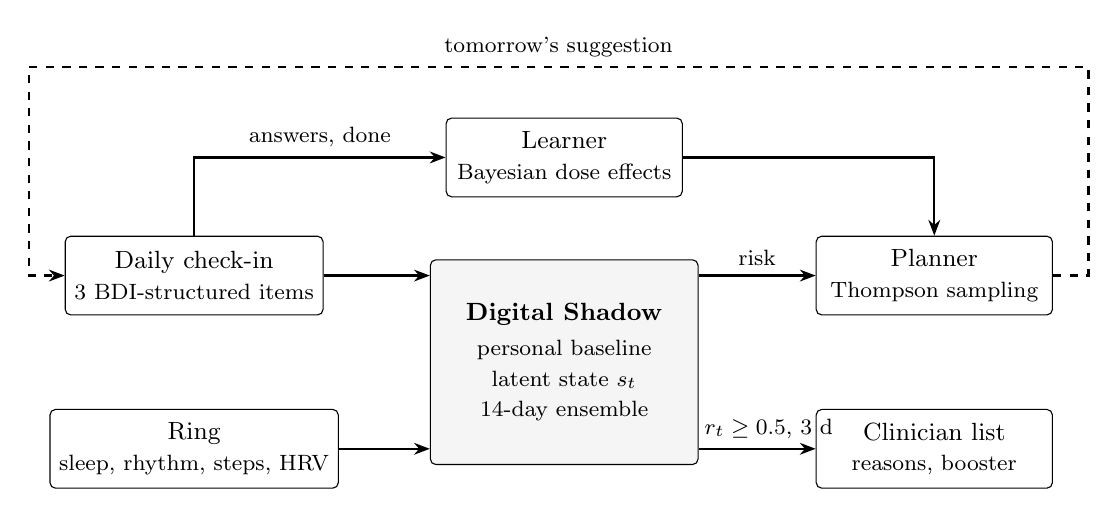
\begin{tikzpicture}[every node/.style={font=\small},
  box/.style={draw, rounded corners=2pt, minimum height=10mm, minimum width=30mm, align=center, fill=white},
  arr/.style={-{Stealth[length=2mm]}, thick}]
\node[box] (ci) at (0,1.1) {Daily check-in\\{\footnotesize 3 BDI-structured items}};
\node[box] (ring) at (0,-1.1) {Ring\\{\footnotesize sleep, rhythm, steps, HRV}};
\node[box, minimum width=34mm, minimum height=26mm, fill=black!4] (shadow) at (4.7,0) {\textbf{Digital Shadow}\\[0.4ex]{\footnotesize personal baseline}\\{\footnotesize latent state $s_t$}\\{\footnotesize 14-day ensemble}};
\node[box] (learn) at (4.7,2.6) {Learner\\{\footnotesize Bayesian dose effects}};
\node[box] (plan) at (9.4,1.1) {Planner\\{\footnotesize Thompson sampling}};
\node[box] (clin) at (9.4,-1.1) {Clinician list\\{\footnotesize reasons, booster}};
\draw[arr] (ci.east) -- (shadow.west |- ci.east);
\draw[arr] (ring.east) -- (shadow.west |- ring.east);
\draw[arr] (shadow.east |- plan.west) -- node[above, font=\footnotesize]{risk} (plan.west);
\draw[arr] (shadow.east |- clin.west) -- node[above, pos=0.6, font=\footnotesize]{$r_t\geq0.5$, 3 d} (clin.west);
\draw[arr] (ci.north) |- node[pos=0.75, above, font=\footnotesize]{answers, done} (learn.west);
\draw[arr] (learn.east) -| (plan.north);
\draw[arr, dashed] (plan.east) -- ++(0.45,0) |- (-2.1,3.75) node[pos=0.75, above, font=\footnotesize]{tomorrow's suggestion} |- (ci.west);
\end{tikzpicture}
\caption{The KEEL loop. Solid arrows run daily. The dashed arrows close the loop: the planner's suggestion reaches the patient, and whether it was done, together with the next check-ins, updates the learner.}
\label{fig:arch}
\end{figure}

\subsection{Data Streams}

Table~\ref{tab:data} lists every input. The model never sees raw text, audio or location.

\begin{table}[h]
\centering\small
\begin{tabular}{@{}lp{6.2cm}p{2.3cm}p{3.2cm}@{}}
\toprule
Stream & Variables & Frequency & Role \\
\midrule
Check-in & 3 of 21 items, score 0--3 each & daily ($\sim$45\,s) & latent state, learner target \\
Adherence & suggestion done / not today & daily, one tap & learner regressor \\
Ring & sleep regularity, relative amplitude, sleep efficiency, wake after sleep onset, steps, nocturnal HRV & nightly / daily & body signal, early warning \\
Clinic & PHQ-9 at end of acute course, booster sessions & events & baseline, intervention \\
\bottomrule
\end{tabular}
\caption{Data used by KEEL.}
\label{tab:data}
\end{table}

\paragraph{Check-in.} The questionnaire follows the structure of the Beck Depression Inventory \cite{beck1961,beck1996}: 21 symptom domains, each answered by choosing the one of four statements that fits best, scored 0--3. The wording is our own; a licensed BDI-II can be substituted item by item. Every item starts from a neutral statement (``I slept about as usual'') and the remaining three describe a change, so no question presumes a bad day. Three items are asked per day on a seven-day rotation, so all 21 domains are covered weekly at about 45 seconds a day. Each item maps onto one of five latent symptom dimensions (Table~\ref{tab:items}). The self-harm item maps onto none: any answer above zero opens a crisis screen with helpline numbers and asks the clinic to call the same day, independent of the model. Dimensions not asked on a given day carry their most recent value forward. The model works on a PHQ-9-equivalent scale, $\mathrm{PHQ}(s) = \tfrac{27}{15}\sum_{d} s_d$ with $s_d \in [0,3]$, so that thresholds are familiar to clinicians.

\begin{table}[h]
\centering\small
\begin{tabular}{@{}lp{11cm}@{}}
\toprule
Latent dimension & Check-in domains (BDI structure) \\
\midrule
Mood & sadness, pessimism, past failure, guilt, punishment feelings, self-dislike, self-criticism, crying, worthlessness \\
Interest & loss of pleasure, loss of interest in others, indecisiveness, concentration, interest in intimacy \\
Sleep & sleep changes \\
Energy & loss of energy, tiredness, appetite changes \\
Anxiety & agitation, irritability \\
Safety only & thoughts of self-harm (crisis path, not modelled) \\
\bottomrule
\end{tabular}
\caption{Mapping of the 21 check-in domains onto the model's five latent dimensions.}
\label{tab:items}
\end{table}

\paragraph{Ring.} Six signals are derived per day. Sleep regularity follows the Sleep Regularity Index; for consumer data we approximate it as $100 - 12\,\mathrm{SD}(\text{mid-sleep}) - 4\,\mathrm{SD}(\text{sleep length})$ over seven nights (hours). Relative amplitude is $(M10-L5)/(M10+L5)$ from the five-minute activity classes, the contrast between the most active ten hours and the least active five. The personal baseline (mean and spread of each signal) is recorded during the last two weeks of the acute rTMS course, when the patient is improving and still under clinical observation.

\subsection{The Mechanistic Patient Model}

Inference and evaluation both rest on a mechanistic model of a post-rTMS patient. Its state lives on five symptom dimensions $d \in \{\text{mood}, \text{interest}, \text{sleep}, \text{energy}, \text{anxiety}\}$. Time is in days from the end of the acute course.

\paragraph{TMS benefit.} The benefit $B_t \in [0,1]$ starts at $B_0 = 1$ and decays toward a personal durable floor $f$ with time constant $\tau$:
\begin{equation}
B_{t+1} = f + (B_t - f)\, e^{-1/\tau}, \qquad f \sim \mathrm{Beta}(2,2), \qquad \log\tau \sim \mathcal{N}(\log 20, 0.9^2).
\end{equation}
A booster block of five sessions sets $B \leftarrow B + 0.8(1-B)$ and adds an acute effect $b=0.7$ per dimension that fades with a 50-day time constant.

\paragraph{Setpoint and symptoms.} Without home support, symptoms head toward the setpoint
\begin{equation}
\mu_t = w + (D - w)(1 - B_t) + (\sigma_t + e_t)\,\ell - b_t,
\end{equation}
where $w$ and $D$ are the personal remission and depressed levels, $\sigma_t$ is a slow Ornstein--Uhlenbeck stress process, $e_t$ are life events (Poisson, rate $1/110$\,d$^{-1}$, exponential size, 21-day decay) and $\ell$ distributes stress over dimensions. Symptoms follow the setpoint slowly and are relieved by the daily activities actually done, $u_t \in \{0,1\}^6$:
\begin{align}
m_{t+1} &= m_t + \alpha_s(\mu_t - m_t) + \eta_t, & \alpha_s &= 0.07\ \text{d}^{-1},\\
E_{t+1} &= E_t + \alpha_u(u_t - E_t), & \alpha_u &= 0.6\ \text{d}^{-1},\\
s_t &= \mathrm{clip}(m_t - W E_t,\ 0,\ 3), & &
\end{align}
where $W \in \mathbb{R}^{5\times 6}$ is the person's hidden response to each activity. Population means of $W$ give 0.5 to 1.4 PHQ-9 points of relief per activity done daily; individual multipliers are log-normal ($\sigma=0.55$) and 20\,\% of person--activity pairs are non-responders. Relapse is defined as a seven-day mean $\mathrm{PHQ}(s) \geq 15$.

\paragraph{Passive signals lead symptoms.} The ring signals respond to the fast-filtered setpoint $p_{t+1} = p_t + \alpha_f(\mu_t - p_t)$, $\alpha_f = 0.3$\,d$^{-1}$, through a fixed linear sensitivity map plus noise. Because $\alpha_f > \alpha_s$, disrupted sleep and rhythm appear before low mood is reported. This encodes the finding of Tonon et al.\ \cite{tonon2026} as an explicit, testable assumption rather than a result of this work.

\paragraph{Calibration.} With no home support, $f$ and $\tau$ were fitted by grid search so that the untreated cohort matches the rTMS durability meta-analysis \cite{senova2019}. The model gives 67.8\,\% and 53.5\,\% relapse-free at 3 and 6 months (published: 66.5\,\% and 52.9\,\%) and 40.7\,\% at 12 months (published: 46.3\,\%); the demonstrator uses the first six months only (Figure~\ref{fig:calib}a).

\subsection{State Estimation and the Two-Week Ensemble Forecast}

Each ring signal $x_{t,j}$ is expressed as an adverse $z$-score against the personal baseline, $z_{t,j} = \pm (x_{t,j} - \bar x_j)/\hat\sigma_j$, with the sign chosen so that positive means worse, and smoothed exponentially, $\tilde z_t = \tilde z_{t-1} + 0.35(z_t - \tilde z_{t-1})$. The \emph{body signal} converts the drift into PHQ-9 points:
\begin{equation}
\hat\mu_t = \mathrm{PHQ}_{\text{well}} + \sum_{j=1}^{6} \beta_j \tilde z_{t,j}, \qquad \beta \geq 0,
\label{eq:body}
\end{equation}
with $\beta$ fitted by non-negative least squares on simulated patient-days ($R^2 = 0.92$; with real paired data this is the component to refit). The reported mood $\hat s_t$ is an exponentially weighted mean of check-ins. The forecast propagates 300 futures for $h = 1,\dots,14$ days:
\begin{align}
\mu^{(i)}_h &= \mu^{(i)}_{h-1} + \kappa\, 0.85^{h} + 0.8\,\xi^{(i)}_h, \qquad \mu^{(i)}_0 = \hat\mu_t,\\
s^{(i)}_h &= s^{(i)}_{h-1} + \alpha_s\big(\mu^{(i)}_h - s^{(i)}_{h-1}\big) + 0.35\,\epsilon^{(i)}_h, \qquad s^{(i)}_0 = \hat s_t,
\end{align}
where $\kappa$ is the damped ten-day slope of $\hat\mu$ and $\xi,\epsilon \sim \mathcal{N}(0,1)$. The spread of the ensemble is the forecast band and the share of futures whose maximum reaches the relapse line is the 14-day risk $r_t$, in the manner of an ensemble weather forecast.

\subsection{Learning What Helps Each Person}

Doses differ in effect between people, so KEEL estimates them per person from that person's own days. The check-in score is modelled as a slow personal baseline minus the effect of recent activity:
\begin{equation}
y_t = \sum_{k} c_k\, h_k(t) - \sum_{a=1}^{6} \theta_a E_{t,a} + \varepsilon_t, \qquad \varepsilon_t \sim \mathcal{N}(0, 1.3^2),
\label{eq:learner}
\end{equation}
where $h_k$ are triangular basis functions with knots every 14 days, so that the natural course of the illness is not credited to an activity, and $E_{t,a}$ is the filtered exposure to activity $a$. The prior on $\theta$ is Gaussian around the population means with standard deviation $0.8\,\theta^{\text{pop}} + 0.4$; the baseline coefficients get a weak smoothness prior. The posterior is available in closed form and is refitted after every check-in in milliseconds.

\paragraph{Planner.} Each of the 63 non-empty subsets $S$ of the six activities is scored on expected relief and effort in minutes; the non-dominated subsets form a Pareto front. Each day a sample $\tilde\theta$ is drawn from the posterior (Thompson sampling \cite{russo2018}) and the plan maximises
\begin{equation}
U(S) = a(|S|)\sum_{k\in S}\tilde\theta_k - \lambda \sum_{k\in S}\text{min}_k, \qquad |S| \leq C(r_t),
\end{equation}
where $a(\cdot)$ is the estimated adherence, which falls as plans grow, and the cap $C$ and effort price $\lambda$ depend on the risk tier (2, 3 or 4 activities for $r_t < 0.15$, $< 0.5$, $\geq 0.5$). Thompson sampling supplies the within-person variation that makes $\theta$ identifiable, while mostly doing what currently looks best.

\paragraph{Escalation.} When $r_t \geq 0.5$ on three consecutive days, the patient moves to the top of the clinic's call list with the reasons (Section~\ref{sec:xai}). In the simulation the clinician accepts and a booster block starts three days later; a 45-day cooldown prevents repeated blocks. The clinician makes every treatment decision.

\subsection{Explaining What Drives the Risk}
\label{sec:xai}

KEEL provides three levels of explanation.

\paragraph{Exact attribution of the body signal.} Equation~\eqref{eq:body} is linear in the smoothed $z$-scores, and the reference point $z=0$ is the person's own baseline. For a linear model, the Shapley values of the features with respect to a reference are exactly $\phi_j = \beta_j(\tilde z_{t,j} - 0)$ \cite{lundberg2017}. The ``reasons'' on the clinician's list (e.g.\ day/night rhythm $-10$\,\%, steps $-23$\,\% against own normal) are these exact attributions translated back into the original units.

\paragraph{TreeSHAP on a risk surrogate.} The full forecast is a non-linear simulation, so we explain it through a surrogate. A gradient-boosted classifier (scikit-learn HistGradientBoosting, 300 iterations) is trained to predict relapse within 14 days from 21 features per patient-day: the six smoothed ring $z$-scores, the five most recent check-in dimensions, 7-day trends of check-ins and body signal, the six activity exposures and days since discharge. Training data are 55\,999 patient-days from 220 simulated patients, each lived under usual care and under the KEEL plan without escalation; 20\,\% of patients are held out. TreeSHAP \cite{lundberg2020} gives exact Shapley values for the surrogate.

\paragraph{Personal dose effects.} The posterior of $\theta$ in Eq.~\eqref{eq:learner} is itself an explanation of what helps this person, with its uncertainty. It is the only one of the three that has a causal reading, because the activity schedule is partly randomised by Thompson sampling.

\section{Evaluation}

All results use simulated patients with seeds disjoint from those used for calibration. Every patient lives the same 180 days (same stress, same life events, same noise) under each of four policies, so differences are due to the policy alone: \emph{usual care} (no home support), a \emph{fixed plan} (morning light and a walk every day), the \emph{KEEL plan} without escalation, and the full \emph{KEEL} loop.

\subsection{A Single Patient}

Figure~\ref{fig:aino} follows one patient, chosen from the simulated cohort because both worlds show the typical pattern clearly. A life event on day 53 disturbs sleep and rhythm; the body signal rises ahead of the check-ins and the forecast crosses the alert threshold on day 59. A booster block on days 62--66 follows. Under usual care the same life leads to relapse on day 89, found at the three-month visit on day 90. With KEEL the peak score is 13.2 and she stays below the relapse line.

\begin{figure}[t]
\centering
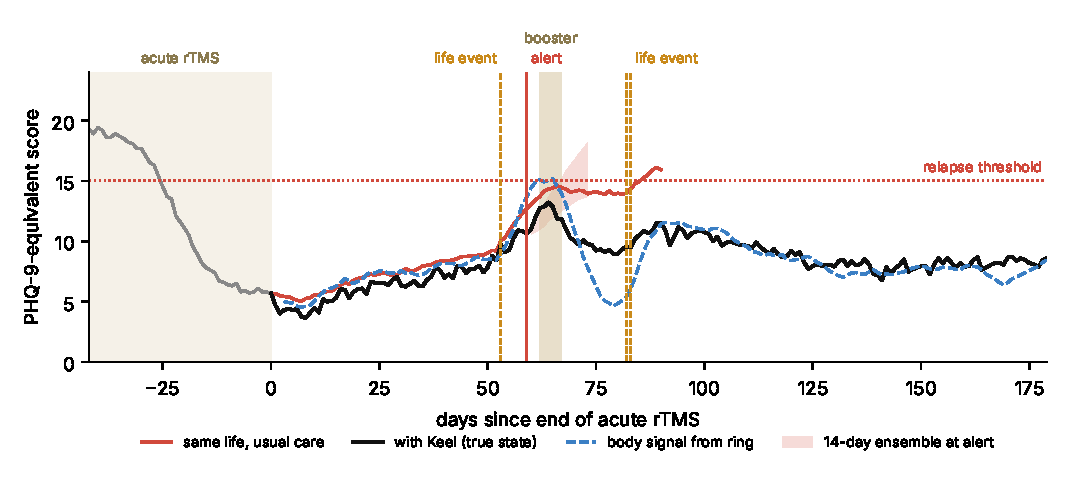
\includegraphics[width=\linewidth]{figures/aino.pdf}
\caption{One simulated patient lived twice. Grey: acute rTMS course. Dashed amber lines: life events. Blue dashed: body signal from the ring, which rises before the reported score. Red band: the 14-day ensemble at the alert. Brass: booster block. Red: the same life under usual care, until the relapse is found at the three-month visit.}
\label{fig:aino}
\end{figure}

\subsection{Cohort Outcomes}

\begin{figure}[t]
\centering
\begin{subfigure}{0.49\linewidth}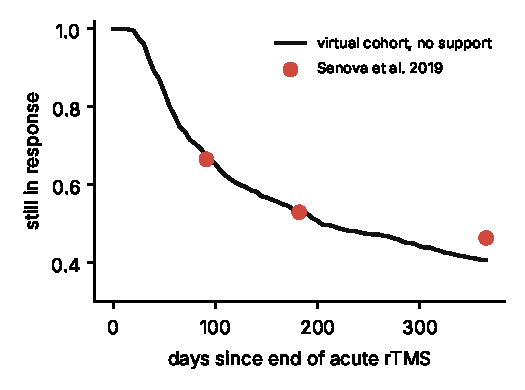
\includegraphics[width=\linewidth]{figures/calibration.pdf}\caption{}\end{subfigure}
\begin{subfigure}{0.49\linewidth}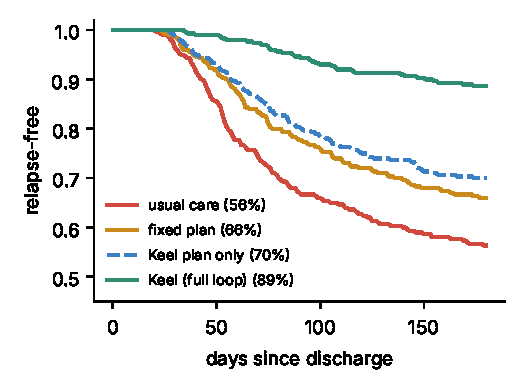
\includegraphics[width=\linewidth]{figures/survival.pdf}\caption{}\end{subfigure}
\caption{(a) Calibration of the untreated virtual cohort ($n=600$) to the rTMS durability meta-analysis \cite{senova2019}. (b) Relapse-free proportion for the same 300 patients under four policies.}
\label{fig:calib}
\end{figure}

\begin{table}[h]
\centering\small
\begin{tabular}{@{}lcccc@{}}
\toprule
Policy & Relapse-free 90 d & Relapse-free 180 d & Days in relapse & Booster blocks \\
\midrule
Usual care & 67.0\,\% & 56.3\,\% & 41.8 & 0 \\
Fixed plan & 77.7\,\% & 66.0\,\% & 29.2 & 0 \\
KEEL plan only & 80.3\,\% & 70.0\,\% & 24.3 & 0 \\
KEEL (full loop) & \textbf{94.7\,\%} & \textbf{88.7\,\%} & \textbf{2.4} & 0.69 \\
\bottomrule
\end{tabular}
\caption{Outcomes over 180 days, 300 simulated patients per policy. Days in relapse: mean days with PHQ-9-equivalent $\geq 15$.}
\label{tab:results}
\end{table}

Table~\ref{tab:results} and Figure~\ref{fig:calib}b summarise the comparison. Personalised daily activities alone improve on usual care and on a fixed plan, but most of the gain comes from timing boosters: the full loop keeps 88.7\,\% of patients relapse-free at six months with 0.69 booster blocks per patient, against six blocks per patient for a monthly fixed schedule. Per patient, KEEL prevented the relapse in 97 of 300, shortened it to less than half in 33, made no difference in 169 who stayed well either way, and failed in one.

\subsection{Early Warning}

\begin{figure}[t]
\centering
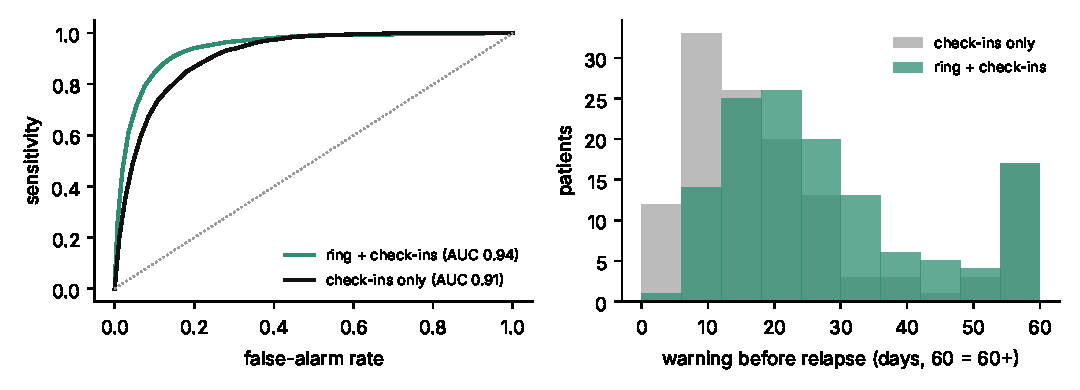
\includegraphics[width=\linewidth]{figures/forecast.pdf}
\caption{Left: ROC of the 14-day risk for days without current relapse, usual-care arm. Right: days between the first warning and the relapse at a matched 10\,\% false-alarm rate (values above 60 pooled).}
\label{fig:forecast}
\end{figure}

Forecast quality is measured on the usual-care arm, where the forecast observes but does not act. For ``relapse within 14 days'' the ensemble reaches AUC 0.94, against 0.91 for the smoothed check-in score alone (Figure~\ref{fig:forecast}). At thresholds chosen for the same 10\,\% false-alarm rate on days that do not precede a relapse, the median warning is 23 days before relapse for ring plus check-ins and 16 days for check-ins alone. The gain is the design assumption of Section~2.3 at work: rhythm changes precede reported mood.

\subsection{Learning}

\begin{figure}[t]
\centering
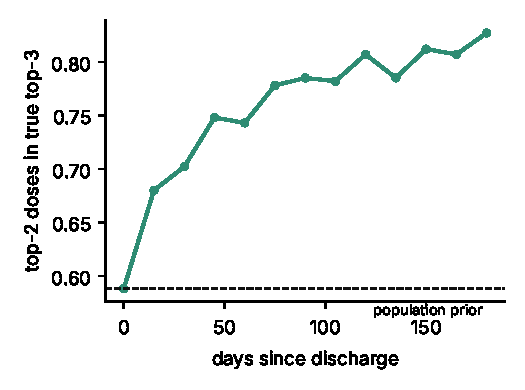
\includegraphics[width=0.55\linewidth]{figures/learning.pdf}
\caption{How often the learner's two favourite activities for a person are among that person's true top three, averaged over 300 patients. Dashed: the population prior used on day 0.}
\label{fig:learning}
\end{figure}

Because activity effects are small relative to day-to-day noise, learning is slow but steady (Figure~\ref{fig:learning}). The share of patients whose two highest-ranked activities are among their true top three rises from 58.8\,\% with the population prior to 82.7\,\% after 180 days, and the mean absolute error of the effect estimates falls from 0.40 to 0.30 PHQ-9 points.

\subsection{What Drives the Risk}

\begin{figure}[t]
\centering
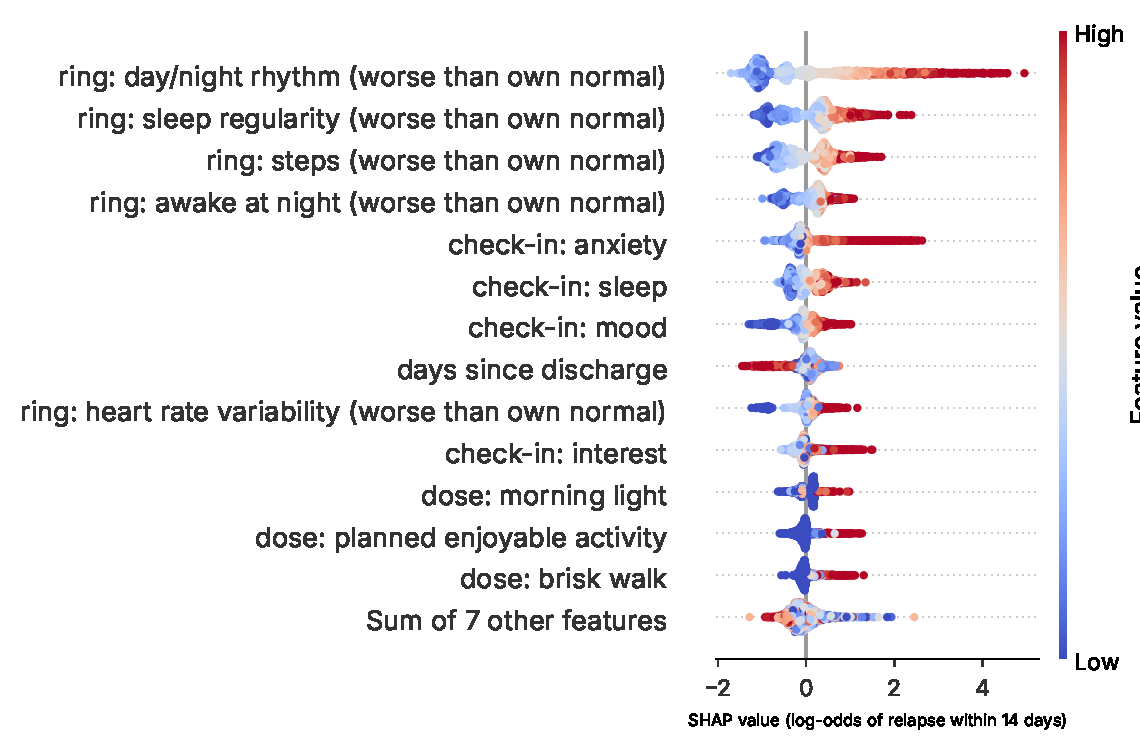
\includegraphics[width=0.9\linewidth]{figures/shap_global.pdf}
\caption{TreeSHAP values of the risk surrogate on held-out simulated patient-days. Each dot is one day; colour is the feature value. Ring features are adverse $z$-scores against the person's own baseline.}
\label{fig:shap}
\end{figure}

The risk surrogate reaches AUC 0.96 on held-out patients. Figure~\ref{fig:shap} ranks its inputs. The largest contributions come from the day/night rhythm (relative amplitude), sleep regularity and steps, each measured against the person's own normal, followed by the check-in dimensions for anxiety, sleep and mood. Days since discharge lowers the risk as time passes, consistent with the decaying hazard of the calibrated cohort.

Two observations need care. First, the ranking reflects the simulator, in which ring signals lead symptoms by design; on real data it is an hypothesis to test, not a finding. Second, higher activity exposure raises the surrogate's risk. This is confounding by indication: the planner prescribes more activities when risk is already high. SHAP explains the surrogate's associations; it does not estimate what an activity does. The causal question is answered by the within-person learner, whose activity schedule is partly randomised.

Figure~\ref{fig:waterfall} explains the alert for the patient of Figure~\ref{fig:aino}. The day before the alert, the flattened day/night rhythm adds 2.5 log-odds, sleep regularity 0.7 and the rising body-signal trend 0.7, while the still-stable check-in trend pulls the risk down by 0.4. This is what the clinician sees as ``why she is on the list''.

\begin{figure}[t]
\centering
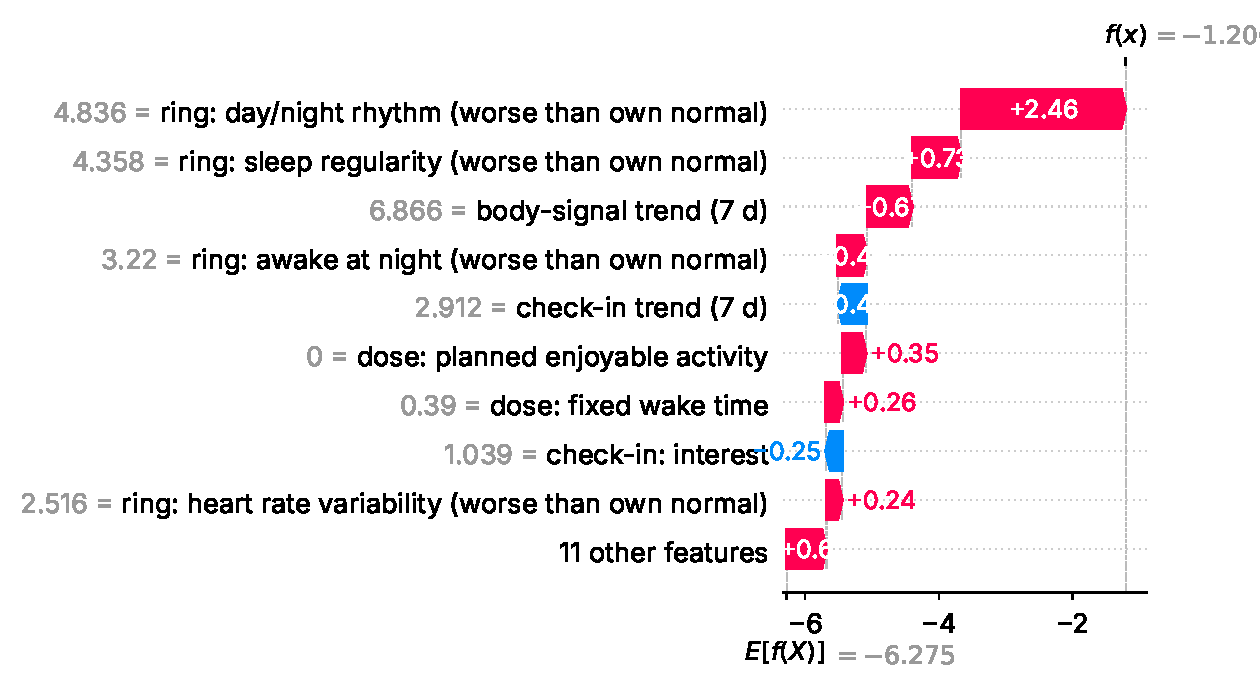
\includegraphics[width=0.9\linewidth]{figures/shap_aino.pdf}
\caption{TreeSHAP explanation of the risk on the day before the alert for the patient of Figure~\ref{fig:aino}, from the base rate $E[f(X)]$ to the prediction $f(x)$ in log-odds.}
\label{fig:waterfall}
\end{figure}

\subsection{Real-Data Check: PSYCHE-D}

The simulator's forecast is an upper bound under its assumptions. To set a floor, we used the public PSYCHE-D dataset \cite{makhmutova2022} (CC BY-NC 4.0): consumer Fitbit features from 8--14 days before a PHQ-9 label, with labels three months apart. Among 7\,291 windows from 3\,069 people who were not depressed at the start (PHQ-9 $<10$; 13\,\% reached PHQ-9 $\geq 10$ three months later), gradient boosting with five-fold cross-validation grouped by person gave AUC 0.60 from wearable features only, 0.79 from the current PHQ-9 only, and 0.78 from both. TreeSHAP on the wearable model ranks moderate-to-vigorous step volume, peak rolling step counts and the variability of sleep duration highest (Figure~\ref{fig:psyched}), which is in line with the activity and regularity features KEEL uses.

\begin{figure}[t]
\centering
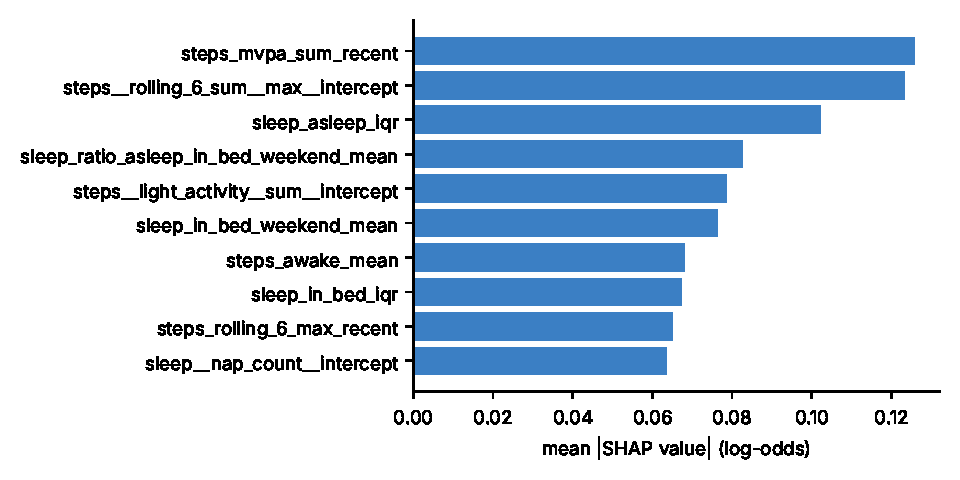
\includegraphics[width=0.85\linewidth]{figures/shap_psyched.pdf}
\caption{Mean absolute TreeSHAP values of the wearable-only model on held-out PSYCHE-D participants.}
\label{fig:psyched}
\end{figure}

A population model on two weeks of consumer data says little three months ahead. KEEL's design responds to this directly: it compares each person with their own baseline instead of with the population, forecasts two weeks rather than three months, always pairs the ring with a daily check-in, and leaves the decision to a clinician.

\section{Discussion and Limitations}

\paragraph{Simulation.} Every outcome in Section~3 except the PSYCHE-D analysis comes from simulated patients. The simulator is calibrated to published relapse rates, but the lead of ring signals over symptoms, the size of activity effects and the effect of a booster block are assumptions. The numbers show that the mechanism works under these assumptions, not that it works in patients.

\paragraph{Check-in instrument.} The items follow the BDI's structure but are not the validated BDI-II and carry its psychometric properties only after validation. Rotating three items a day trades completeness on any single day for low burden; the carry-forward of unasked dimensions delays the response to change by up to a week, which the ring partly compensates.

\paragraph{Patient-facing design.} The relapse probability is shown only to the care team. Patients see their week against their usual and the activities that have helped them, and can switch on a neutral two-week outlook together with their clinician. This choice follows concerns about emotional burden in remitted patients \cite{coenen2025} and should itself be tested.

\paragraph{Next steps.} A pilot at an rTMS clinic would equip patients with a ring from the last week of the acute course, collect daily items for six months alongside the clinic's usual follow-up, refit the body-signal weights $\beta$ on real paired data, and compare the warnings with clinician-rated relapse. TMS-EEG or resting EEG recorded in the clinic could provide a further baseline for the personal model.

\section{Conclusion}

KEEL turns maintenance after rTMS from a fixed calendar into a forecast. A mechanistic Digital Shadow, fed by three neutral questions a day and a ring, estimates each patient's state against their own normal, forecasts relapse two weeks ahead, learns which everyday activities help that person, and tells the clinician who needs a booster and why. In a simulated cohort calibrated to rTMS durability, the loop raised the six-month relapse-free proportion from 56\,\% to 89\,\% with fewer than one booster block per patient, and warned a median of 23 days ahead. Exact additive attributions and TreeSHAP make each warning inspectable, and a check on real consumer-wearable data defines where the method must improve before clinical use.

\section*{Code Availability}

The simulator, forecast, learner, evaluation scripts, the figure pipeline for this paper (\texttt{paper\_figures.py}) and the demonstrator (patient phone, clinician list, evidence view) are available at\\ \url{https://github.com/Latt33/keel}.

\FloatBarrier
\begin{thebibliography}{99}\small
\bibitem{senova2019} S.~Senova, G.~Cotovio, A.~Pascual-Leone, A.~J.~Oliveira-Maia. Durability of antidepressant response to repetitive transcranial magnetic stimulation: systematic review and meta-analysis. \emph{Brain Stimulation}, 12(1):119--128, 2019.
\bibitem{akram2024} S.~Akram, I.~Nanji, I.~Deniz, F.~Akram, F.~Mukhtar. Maintenance repetitive transcranial magnetic stimulation for major depressive disorder. \emph{The Journal of ECT}, 2024. doi:10.1097/YCT.0000000000001064.
\bibitem{tonon2026} A.~C.~Tonon, A.~Nexha, J.~E.~A.~Cunningham, et al. One-year actigraphy study of sleep and rest-activity rhythms as markers of relapse in depression. \emph{JAMA Psychiatry}, 2026. doi:10.1001/jamapsychiatry.2025.4453.
\bibitem{makhmutova2022} M.~Makhmutova, R.~Kainkaryam, M.~Ferreira, J.~Min, M.~Jaggi, I.~Clay. Predicting changes in depression severity using the PSYCHE-D model involving person-generated health data: longitudinal case-control observational study. \emph{JMIR mHealth and uHealth}, 10(3):e34148, 2022.
\bibitem{niederer2021} S.~A.~Niederer et al. Scaling digital twins from the artisanal to the industrial. \emph{Nature Computational Science}, 1(5), 2021.
\bibitem{laakso2026} A.~Laakso, M.~Chen, N.~Juhava, Q.~Li. STIMIQ: a digital shadow architecture for deep brain stimulation optimization via amortized inference. Technical report, 2026. \url{https://github.com/Latt33/StimIQ}.
\bibitem{coenen2025} T.~Coenen et al. Requirements and concerns of individuals remitted from depression for an early relapse detection mHealth app: focus group study. \emph{JMIR mHealth and uHealth}, 13:e67141, 2025.
\bibitem{beck1961} A.~T.~Beck, C.~H.~Ward, M.~Mendelson, J.~Mock, J.~Erbaugh. An inventory for measuring depression. \emph{Archives of General Psychiatry}, 4:561--571, 1961.
\bibitem{beck1996} A.~T.~Beck, R.~A.~Steer, G.~K.~Brown. \emph{Manual for the Beck Depression Inventory-II}. Psychological Corporation, San Antonio, 1996.
\bibitem{russo2018} D.~J.~Russo, B.~Van~Roy, A.~Kazerouni, I.~Osband, Z.~Wen. A tutorial on Thompson sampling. \emph{Foundations and Trends in Machine Learning}, 11(1):1--96, 2018.
\bibitem{lundberg2017} S.~M.~Lundberg, S.-I.~Lee. A unified approach to interpreting model predictions. \emph{Advances in Neural Information Processing Systems}, 30, 2017.
\bibitem{lundberg2020} S.~M.~Lundberg et al. From local explanations to global understanding with explainable AI for trees. \emph{Nature Machine Intelligence}, 2(1):56--67, 2020.
\end{thebibliography}

\end{document}
